%%%%%%%%%%%%%%%%%%%%%%%%%%%%%%%%%%%%%%%%%%%%%%%%%%%%%%%%%%%%%%%
\section{Simulation and Physics}
\label{sec:fdsp-pd-simphys}
%\metainfo{(Length: TDR=50 pages, TP=20 pages)}
%\metainfo{\color{blue} Content: Conveners}


The potential physics performance of photon detector designs is evaluated using a full simulation, reconstruction, and analysis chain developed for the LArSoft framework. The goal is to evaluate the performance in physics deliverables of the range of design possibilities under consideration. The metrics evaluated will include efficiency for determining T0, timing resolution, and calorimetric energy resolution for three physics samples: supernova neutrinos, nucleon decay events\footnote{The most relevant sample is actually the \emph{background} to nucleon decay events. However, efficiently simulating background which can mimic nucleon decays is challenging since they can be quite rare topologies, so it is easier to simulate the nucleon decay signal which must be representative of the background.}, and beam neutrinos. However, the development of analysis tools to take advantage of this full simulation chain is fairly recent, so this proposal will only include one test case: T0-finding efficiency for supernova neutrinos vs. the ``effective area'' of the photon collectors.

The first step in the simulation specific to the photon detection system is the simulation of the production of light and its transport within the volume to the photon detectors. Argon is a strong scintillator, producing \SI{24000}{$\gamma$s/MeV} at our nominal drift field. Even accounting for the efficiency of the photon detectors, it is prohibitive to simulate every optical photon with Geant4 in every event. So, in advance the detector volume is voxelized and many photons are produced in each voxel. The fraction of photons from each voxel reaching each photosensor is called the ``visibility,'' and these visibilities are recorded in a 4-dimensional library (akin to the ``photon maps'' used in the dual phase simulation). This library includes Rayleigh scattering ($\lambda=$ \SI{55}{cm}), absorption ($\lambda=$ \SI{20}{m}), and the measured collection efficiency vs. position of the double-shift light-guide bars. When a particle is simulated, at each step it produces charge and light. The light produced is distributed onto the various photon detectors using the photon library as a look-up table and the early (\SI{6}{ns}) plus late (\SI{1.6}{$\mu$s}) scintillation time constants are applied. Transport time of the light through the argon is not currently simulated, but is under development.

The second step is the simulation of the electronics response. Waveforms are produced on each channel by adding an SiPM single-PE response shape for each true photon. In addition, other electronics ``imperfections'' are added. Dark noise, at a rate of \SI{10}{Hz} for each of the three SiPM's on each channel is added by adding additional single-PE waveforms. Crosstalk (where a second cell avalanches when a neighbor is struck by a photon) is introduced by adding a second PE \num{16.5}\% of the time when an initial PE is added to the waveform. Additional uncorrelated random noise is added to the waveform with an RMS of \SI{2.6}{ADC} (or approximately \SI{0.1}{PE}). The response of the SSP self-triggering algorithm, based on a leading-edge discriminator, is then simulated to determine if and when a \SI{7.8}{$\mu$s} waveform will be read out, or in the case of the simulation stored and passed on for later processing.

The third step is reconstruction, which proceeds in three stages. The first is a ``hit finding'' algorithm which searches for peaks on individual waveforms channel-by-channel, identifying the time based on the time of the first peak and the total amount of light collected based on the integral until the hit goes back below threshold. The second step is a ``flash finding'' algorithm which searches for coincident hits across multiple channels. All the coincident light is collected up into a single object which has an associated time (the earliest hit), an amount of light (summed from all the hits), and a position on the plane of the APAs (Y-Z) which is a weighted-average of the positions of the photon collectors with hits in the flash\footnote{Right now the flash reconstruction does not consider the positions of the hits, only their times. This will need to be updated in the future when we simulate the full-sized far detector, but for now we are working in a small test geometry which acts as a crude simulation of this kind of constraint.}. The final step is to ``match'' the flash to the original event by taking the largest flash within the allowed drift time which is within \SI{240}{cm} in the Y-Z plane. Since the TPC reconstruction is still in active development, especially for low energy events, we match to the true MC vertex of the event in the analyses presented here. We believe this is a reasonable approximation since the position resolution of the TPC will be \emph{significantly} better than that of the photon detection system. 

\begin{dunefigure}[Efficiency for finding T0 for supernova neutrino events vs. the effective area of the photon detection system. NOTE: numbers are not final.]{fig:pds-snefficiency}
{Efficiency for finding T0 for supernova neutrino events vs. the effective area of the photon detection system. NOTE: numbers are not final.}
  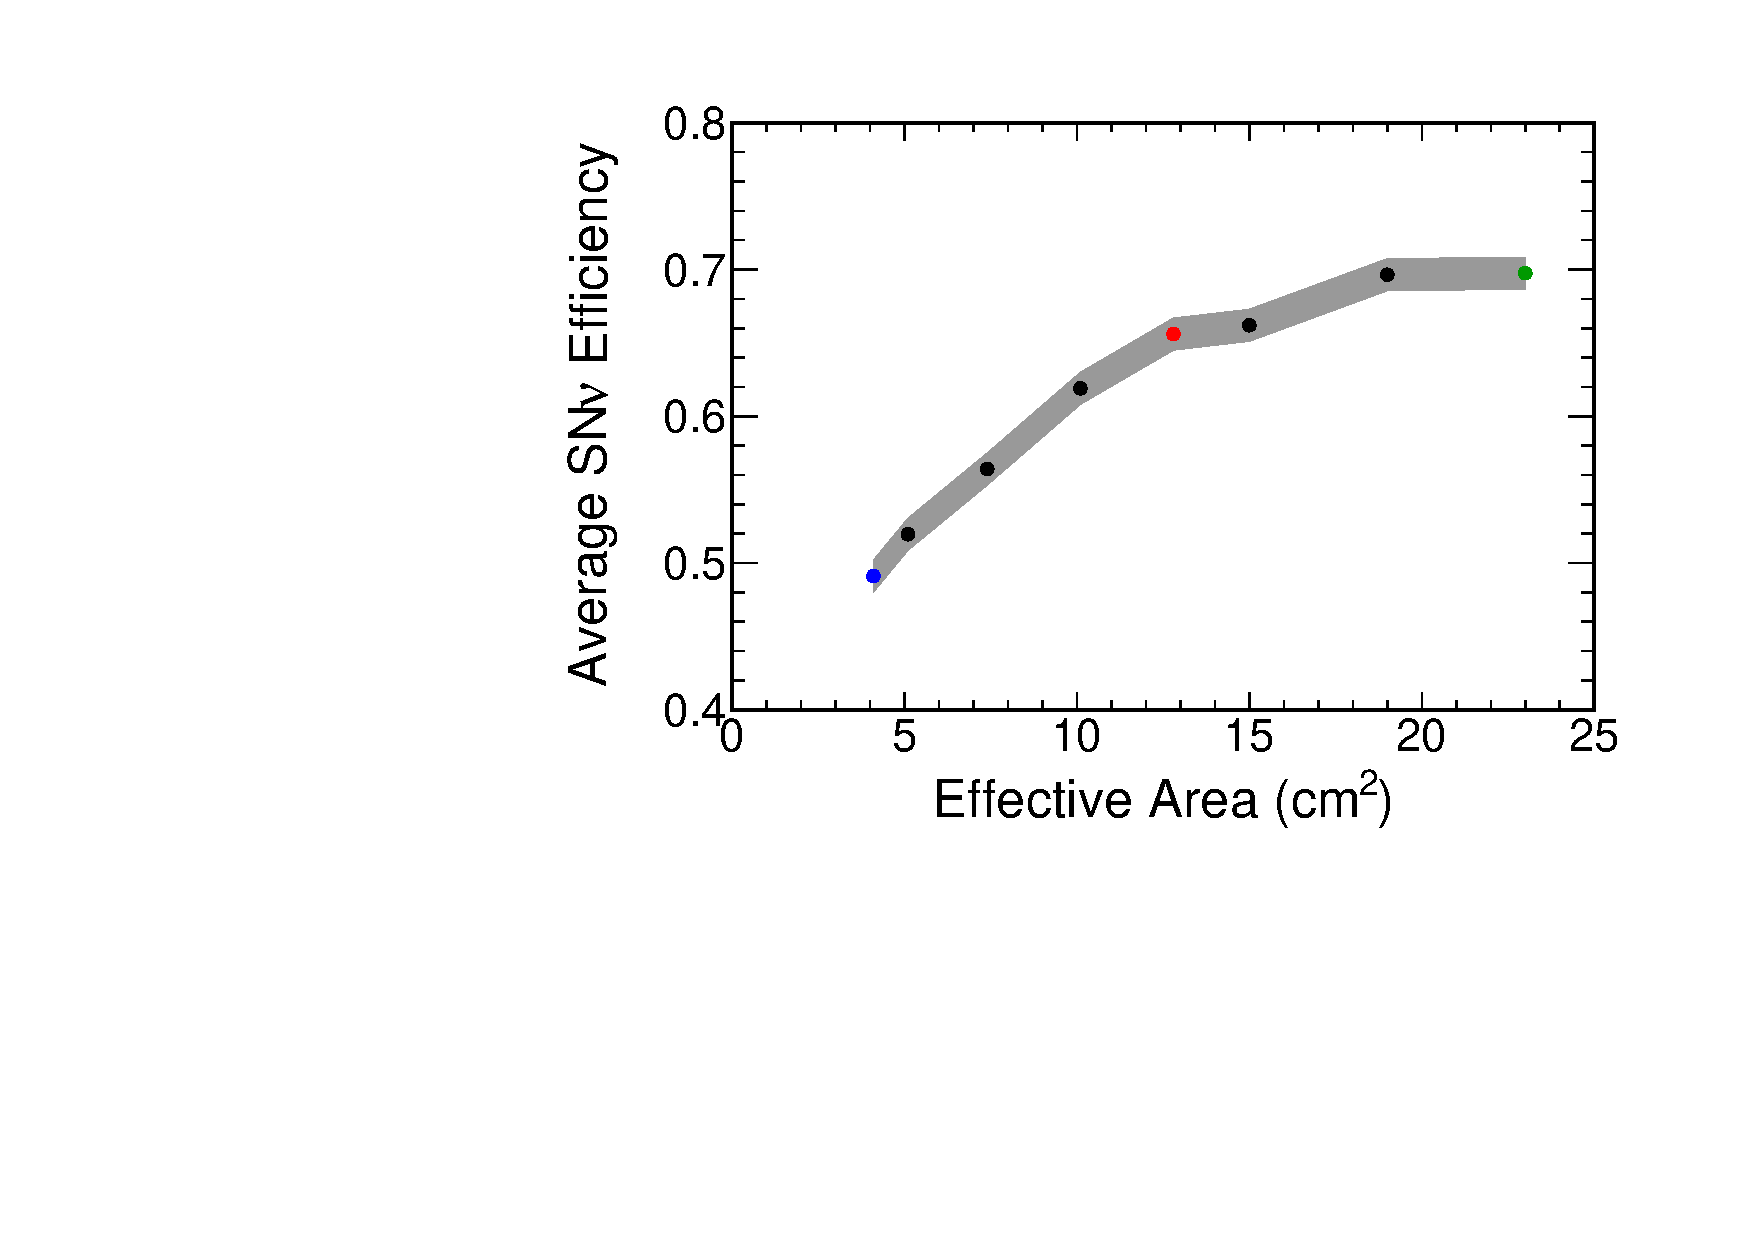
\includegraphics[width=0.6\columnwidth]{pds-efficiency.pdf}
\end{dunefigure}

\begin{dunefigure}[Efficiency for finding T0 for supernova neutrino events vs. distance from the andode plane. NOTE: numbers are not final.]{fig:pds-sneff-x}
{Efficiency for finding T0 for supernova neutrino events vs. distance from the andode plane. NOTE: numbers are not final.}
  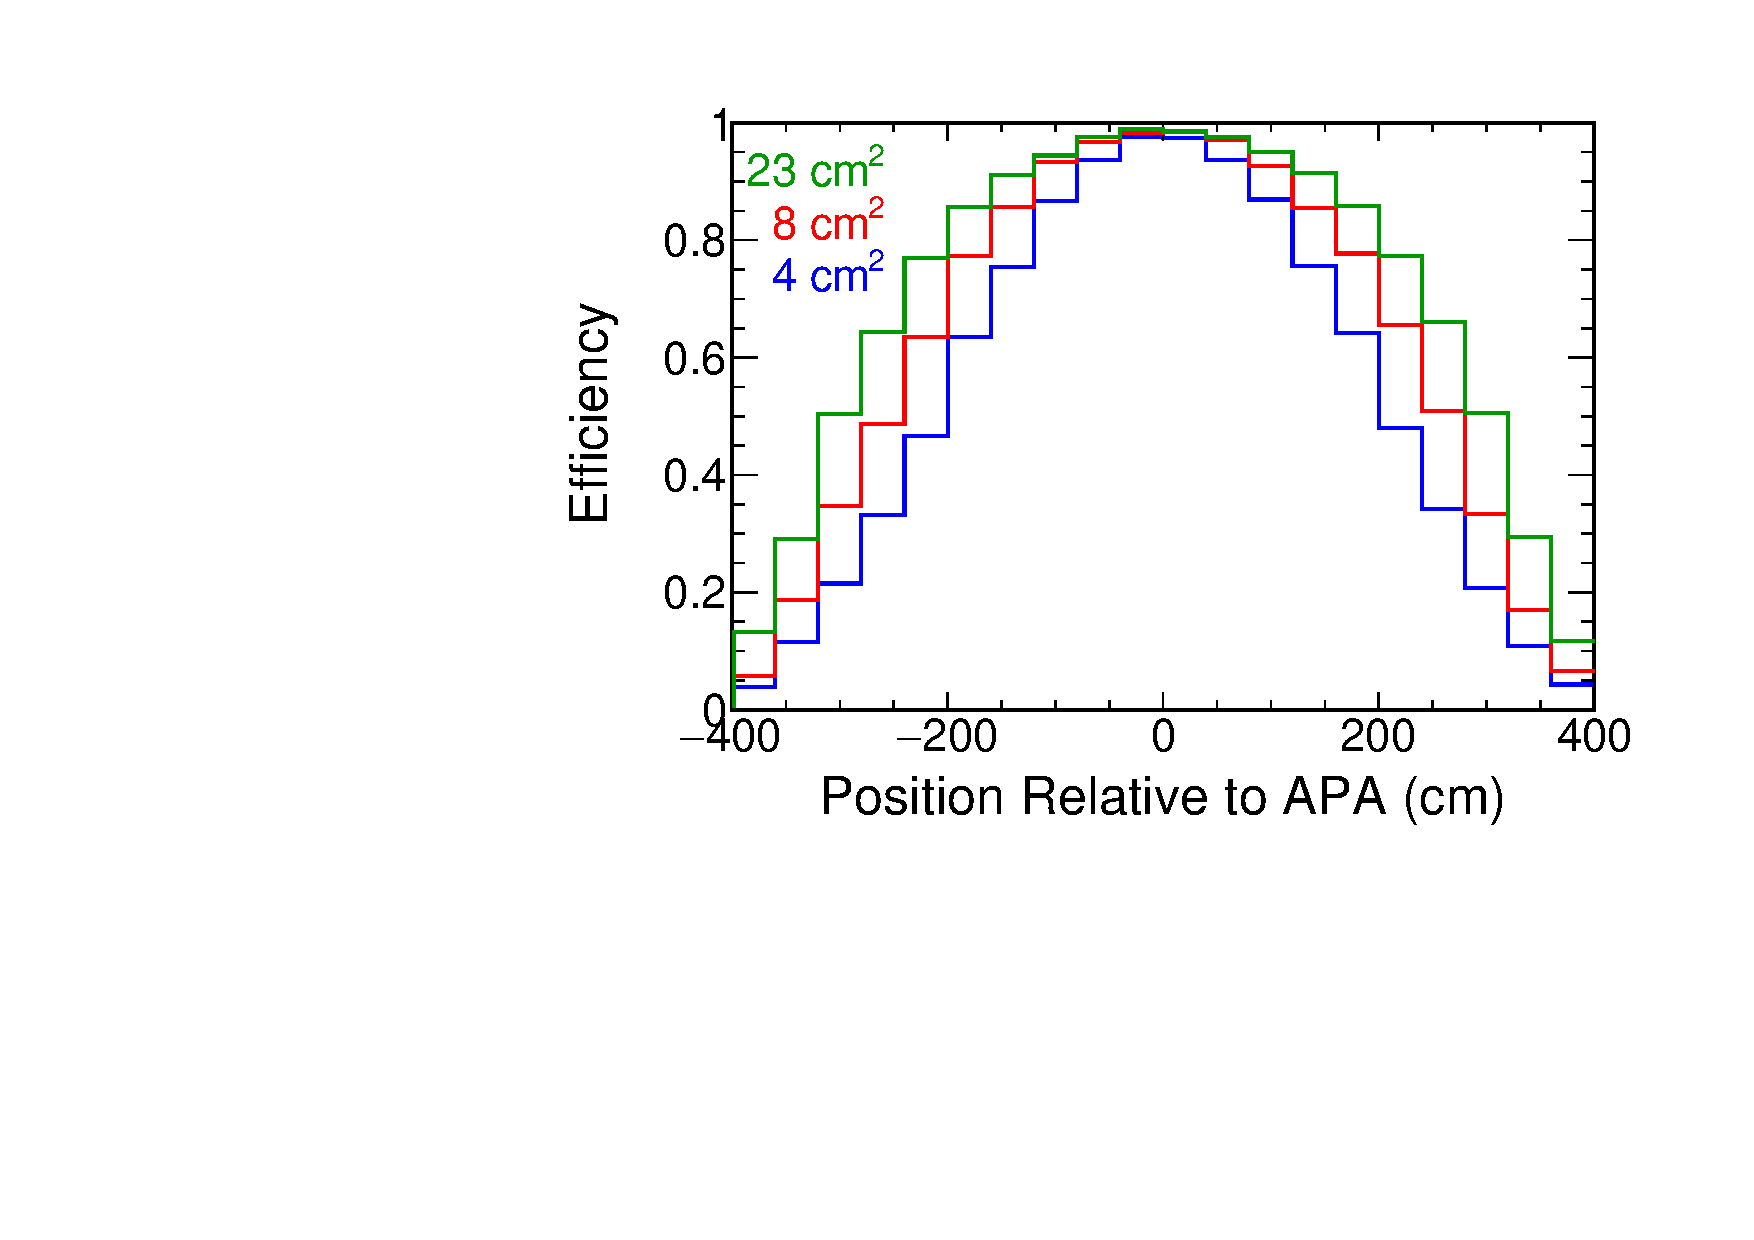
\includegraphics[width=0.6\columnwidth]{pds-position.pdf}
\end{dunefigure}

\begin{dunefigure}[Efficiency for finding T0 for supernova neutrino events vs. neutrino energy. NOTE: numbers are not final.]{fig:pds-sneff-e}
{Efficiency for finding T0 for supernova neutrino events vs. neutrino energy. NOTE: numbers are not final.}
  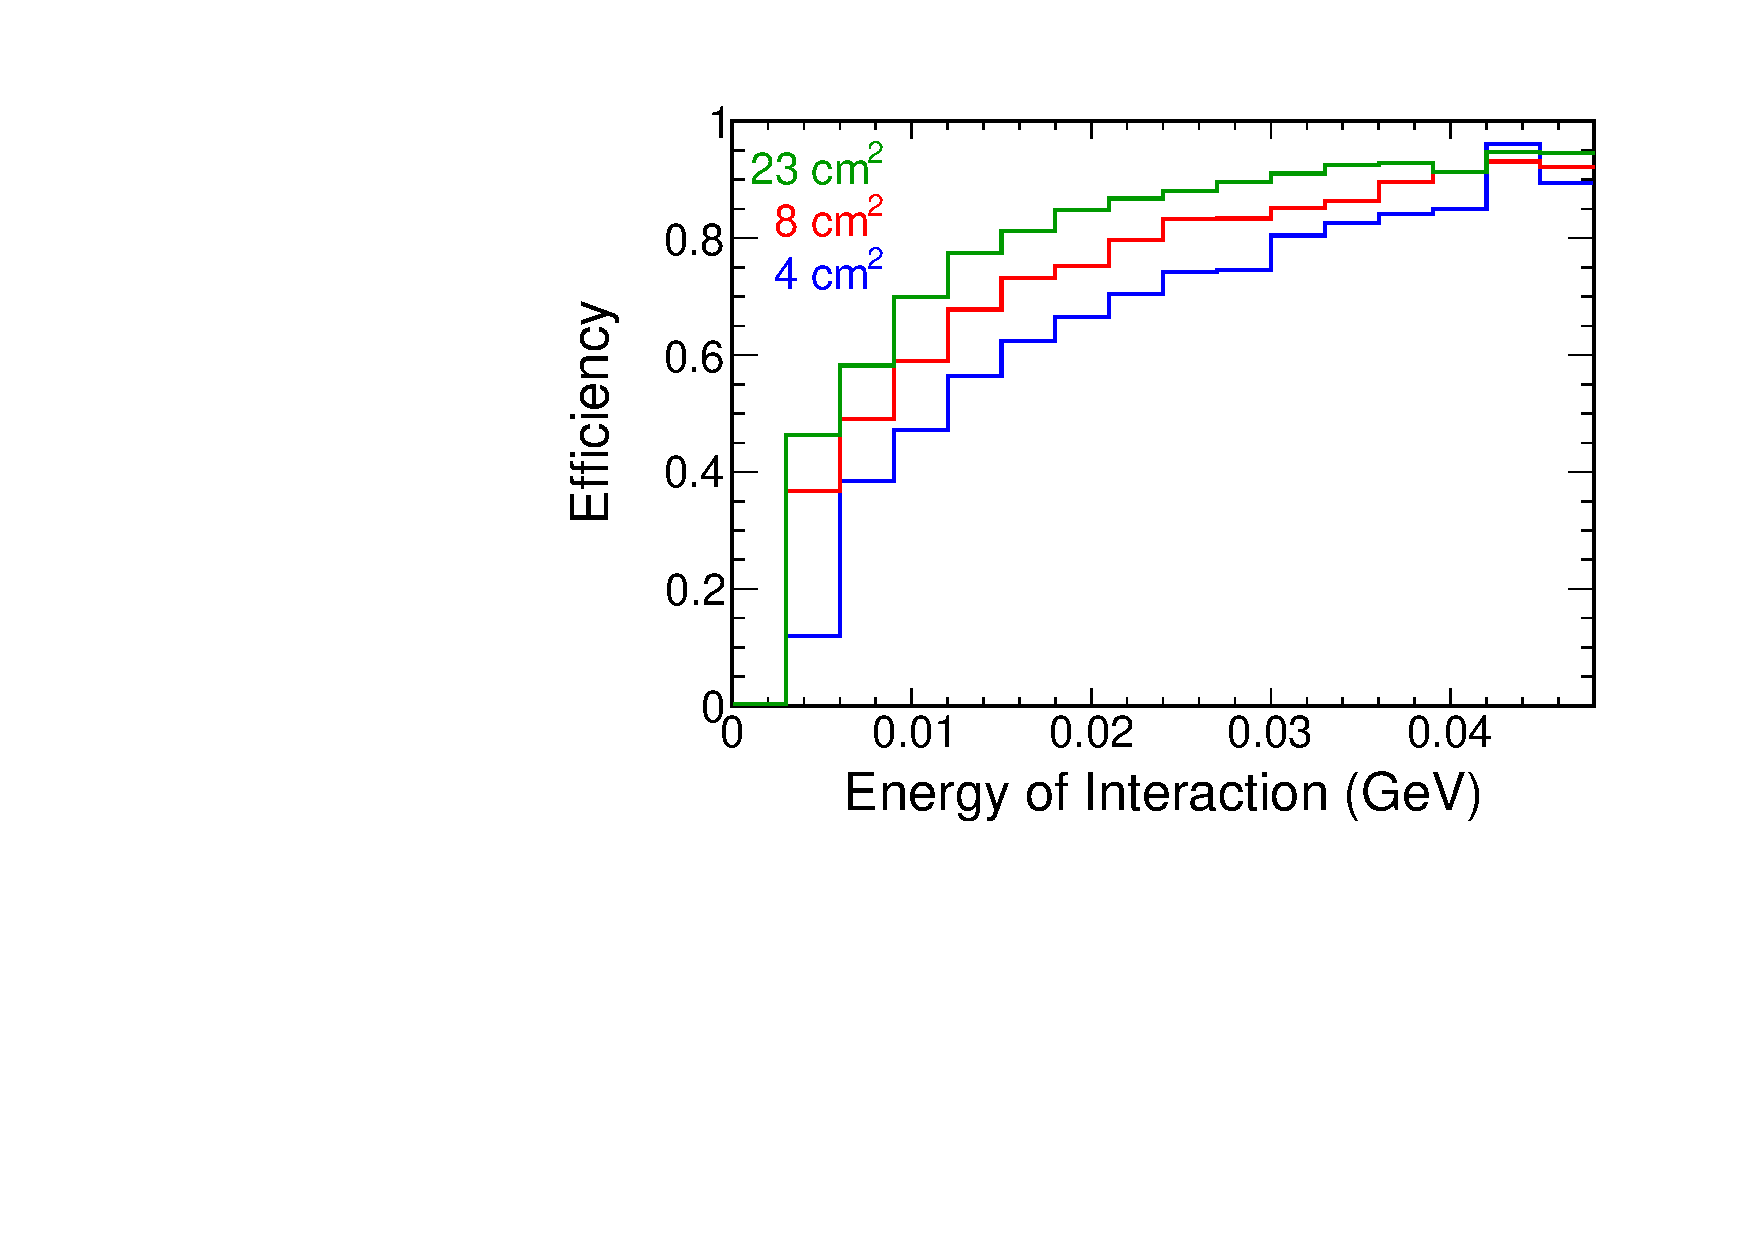
\includegraphics[width=0.6\columnwidth]{pds-energy.pdf}
\end{dunefigure}

Figure~\ref{fig:pds-snefficiency} shows the efficiency for determining T0 for events in a typical supernova spectrum using the tools above. The changes in effective areas which could correspond to alternative photon collection designs are achieved by simply scaling up the total efficiency of the simulated double-shift light guide design. The differences in attenuation behaviors within the bars are a second-order effect relative to the total amount of light collected. The efficiency for finding T0 for these events increases linearly up through about \SI{15}{cm^2} of effective area, at which point the gains begin to slow down. Figures~\ref{fig:pds-sneff-x} and~\ref{fig:pds-sneff-e} show how the efficiency varies vs. neutrino energy and distance from the anode plane for three chosen points.
